
El cáncer\index{Cáncer} es, por definición, un conjunto de enfermedades con diferentes
localizaciones dentro del cuerpo, diferentes síntomas y causas. Todos los tipos
de cáncer comparten una característica, que es la replicación descontrolada de
ciertas células dentro del cuerpo, esta replicación ocurre en todas partes del
cuerpo de manera natural y es el sistema inmunológico el que se encarga de
eliminar estas réplicas extrañas. El problema radica en que a veces la tasa de
réplica es mayor a la tasa de eliminación, las células cancerígenas también
pueden inhibir y combatir la acción del sistema inmune. Son estas variables las
que hacen del cáncer un flagelo para la vida humana.

La enfermedad puede manifestarse en casi cualquier parte del cuerpo y se
manifiesta, generalmente, formando tumores sólidos\index{Tumor}, que no son
más que agregados de células cancerígenas. Estos tumores crean vasos sanguíneos
e infraestructuras para su alimentación, lo que causa problemas sistémicos
dentro del cuerpo. La diferencia entre los tumores cancerígenos (malignos) y
otros tipos de tumores (benignos) es que el cáncer se expande e invade tejidos,
comenzando por los más cercanos para luego invadir estructuras alejadas del
origen.

El cáncer es una enfermedad de origen genético, dentro de las células existen
moléculas y proteínas especiales que dictan su comportamiento metabólico. Estas
moléculas y proteínas reciben el nombre de \hyperlink{abbr}{ADN}. Esto es lo que
se daña dentro de las células y es lo que conlleva al desarrollo del cáncer. Las
células enfermas difieren de las sanas en su tasa de replicación y su
inmortalidad.

Las causas del cáncer son variadas y dependen de la forma en que se realiza este
daño genético. El cáncer o la propensión a este se puede heredar, condiciones
ambientales y exposición a agente como químicos también inciden en la
probabilidad de generar cáncer. Otros factores incluyen la alimentación, hábitos
y vicios, exposición al sol etcétera. Los cambios de las células, cuando son
anormales e indicadores de cáncer, se llaman Displasias\index{Displacia} (del
griego antiguo \textdelta\textupsilon\textvarsigma, `dys', dificultad, y el
sufijo -plasia derivado del verbo
\textpi\textlambda\textalpha\textsigma\textsigma\textomega, `plásso', formar).
El estado previo al daño causante de cáncer se conoce como hiperplasia y este no
siempre se manifiesta en cáncer.

Existen muchísimos tipos de cáncer, es probable que más de 100. Estos se nombran
tradicionalmente en función al órgano o tejido afectado. Pero no se limitan a
estos órganos, puesto que los cánceres pueden migrar, generalmente se nombran
por el órgano afectado inicial.

El tipo de cáncer más común es el carcinoma\index{Carcinoma}. Cuyo origen son
las células epiteliales, células que fungen como capa externa de todas las
superficies corporales, tanto internas como externas. Debido a su alto grado de
exposición al ambiente, son estas células las más propensas a sufrir mutaciones.
Distintos tipos de daños causan distintos tipos de carcinomas epiteliales, por
ejemplo el adenocarcinoma se produce cuando las células dañadas son aquellas que
producen fluidos dentro del cuerpo; el carcinoma de células escamosas ocurre en
las células que están directamente debajo de las capas exteriores de la piel y
tejidos externos, como las paredes del ano o
vaginales.~\cite{NationalCancerInstitute}

\subsection{Historia y causas}

La palabra cáncer tiene su raíz etimológica de la palabra griega
\textkappa\textalpha\textrho\textkappa\textiota\textnu\textomikron\textvarsigma,
`karkinos' que significa cangrejo y fue utilizada por Hipócrates (460-370 A.C)
para describir tumores cancerígenos, sin embargo, existe evidencia de que él no
fue el primero en describir la enfermedad. Algunas evidencias tempranas de
cáncer de hueso fueron encontradas en momias del antiguo Egipto y en manuscritos
que datan del 1600 A.C. El registro más viejo de algún caso de cáncer de mama
proviene del año 1500 A.C en Egipto y se registró que no se tenía conocimiento
de cura para tal padecimiento, solo tratamiento paliativo podría ser aplicado al
paciente. Así mismo, se tiene certeza en ciertas escrituras e inscripciones, que
algunos tumores superficiales eran extirpados quirúrgicamente por la incipiente
medicina de aquél tiempo.~\cite{AmericanCancerSocietyb}

\subsubsection{Causas genéticas}

Existen dos tipos principales de genes que tienen importantes roles en el cáncer

\begin{itemize}
    \item{Oncogenes}: Proto-oncogenes son aquellos genes que ayudan a una célula
    a crecer. Cuando un oncogén muta o hay demasiadas copias de él mismo, se
    convierte en un gen atrofiado que puede activarse permanentemente o
    activarse cuando se supone que no debería estar activo. Cuando esto sucede,
    la célula crece sin control, lo que puede derivar en cáncer. A esto se le
    conoce como oncogén. Algunos cánceres son causados por mutaciones heredades
    de estos proto-oncogenes que causan activación de un oncogén en particular;
    pero la mayoría de los cánceres que involucran tales oncogenes son
    adquiridos no heredados.
    \item{Genes supresores}: Son genes normales que reducen la velocidad de
    replicación celular, reparan errores en el \hyperlink{abbr}{ADN} o indican el final del ciclo
    de vida celular, proceso conocido como apoptosis o muerte celular
    programada. Cuando los genes supresores no actúan correctamente, las células
    pueden crecer sin control alguno, lo que derivaría en cáncer. La diferencia
    entre estos y los oncogenes, es que los oncogenes causan cáncer cuando se
    activan, mientras que los genes supresores lo causan cuando se desactivan.
    Algunas anomalías heredadas en los supresores de tumores han sido
    encontradas en algunas familias de cáncer. Estas convierten a estos tipos de
    cáncer en ubicuos para determinada familia, pero la mayoría de los genes
    supresores de tumores son adquiridos, no heredados.
\end{itemize}

\subsubsection{Causas ambientales}

La mitad de las causas genéticas de cáncer no son genes heredados sino
adquiridos del medio ambiente. Estos elementos del ambiente, llamados
carcinógenos no necesariamente dañan los genes directamente, por ejemplo, pueden
incidir en la velocidad de replicación de una célula y esto incrementa la
probabilidad de mutaciones en la misma:

\begin{minipage}{\textwidth}
\begin{itemize}
    \item{Estilo de vida}: Nutrición, uso de tabaco, falta de actividad física
    \item{Exposiciones naturales}: Luz ultravioleta, gas radón, radiación
    cósmica.
    \item{Tratamientos médicos}: quimioterapia, radiación, hormonas,
    medicamentos supresores del sistema inmune.
    \item{Exposición laboral}: Elementos químicos, asbesto, mercurio-
    \item{Exposición en el hogar}: Detergentes, pesticidas, empaques de
    alimentos.
    \item{Contaminación}: Smog, metales pesados, daño en la capa de ozono.     
\end{itemize}
\end{minipage}

Los carcinógenos se clasifican de la siguiente manera:
\begin{itemize}
    \item{\textbf{Grupo 1: }} Carcinógeno para humanos
    \item{\textbf{Grupo 2A: }} Probable carcinógeno para humanos
    \item{\textbf{Grupo 2B: }} Posible carcinógeno para humanos.
    \item{\textbf{Grupo 3: }} Inclasificable como carcinógeno para humanos.
    \item{\textbf{Grupo4: }} Probablemente no carcinógeno para humanos.  
\end{itemize}

Como se puede observar, no hay una categoría específica para elementos 100\%
seguros y libres de potencial cancerígeno. Todo contacto con el medio ambiente
es capaz de detonar los cambios y daños celulares requeridos para detonar un
cáncer.

\subsubsection{Causas infecciosas}

Desde principios del siglo XX, se ha conocido que ciertas infecciones juegan un
rol en incitar cáncer en animales. Recientemente, infecciones de ciertos virus,
bacterias y parásitos han sido reconocidas como factores de riesgo para varios
tipos de cáncer+ en humanos. Las infecciones pueden elevar el riesgo de padecer
cáncer en una persona de distintas maneras, por ejemplo:

\begin{enumerate}
    \item Algunos virus afectan directamente los genes dentro de las células que
    controlan su crecimiento. Estos virus pueden insertar sus propios genes
    dentro de la célula, causando a la célula crecer sin control.
    \item Infecciones pueden causar inflamación crónica en ciertas partes del
    cuerpo. Esto puede llevar a cambios en las células afectadas y en células
    inmunes cercanas, que eventualmente se pueden derivar en cáncer.
    \item Cierto tipo de infecciones pueden suprimir el sistema inmune de una
    persona, el cual normalmente ayuda a proteger al cuerpo de algunos cánceres.
\end{enumerate}

Si bien este tipo de infecciones pueden elevar el riesgo personal a padecer
cáncer, en la mayoría de los casos las personas infectadas nunca desarrollan
cáncer. El riesgo de desarrollarlo depende también de otros factores. Por
ejemplo, infección estomacal por Helicobacter Pylori puede incrementar el riesgo
de cáncer de estómago; pero también que se come, si se fuma o no y otros más
factores que inciden en el riesgo. 

Los virus son agentes infecciosos diminutos capaces de infectar células y
cambiar su \hyperlink{abbr}{ADN}. Es esta afectación del \hyperlink{abbr}{ADN}
(y del ARN) que puede desencadenar varios tipos de cáncer. Muchos virus son
capaces de generar cáncer en los seres humanos, empero, cada virus infecta
generalmente un solo tipo de célula dentro del cuerpo humano. Actualmente se
trabajan en medidas preventivas como vacunas para reducir la incidencia de
cáncer causado por infecciones. 

\subsection{Cáncer cérvico-uterino}

El cáncer cervicouterino\index{Cáncer cérvico-uterino} es aquel cáncer que se
presenta en el cuello uterino o cérvix, por ello es un cáncer exclusivo de la
población femenina. El cuello uterino es una parte del sistema reproductor de la
mujer y se encuentra en la pelvis, el extremo del útero que está en contacto con
la vagina. La mayoría de los estudios apunta a una causa general del cáncer de
cérvix. La presencia de Virus de Papiloma Humano es el desencadenante de las
mutaciones que general la replicación descontrolada de las células del cérvix,
es decir, el cáncer. Otros factores de riesgo incluyen los tradicionales de
cualquier cáncer, como tabaquismo, así como factores específicos como la edad,
parejas sexuales, predisposición genética y otros más. En
la~\autoref{fig:cervix} se ve la posición anatómica y relativa del cervix con
respecto al cuerpo femenino y al aparato reproductor.

\begin{figure}[H]
    \centering
    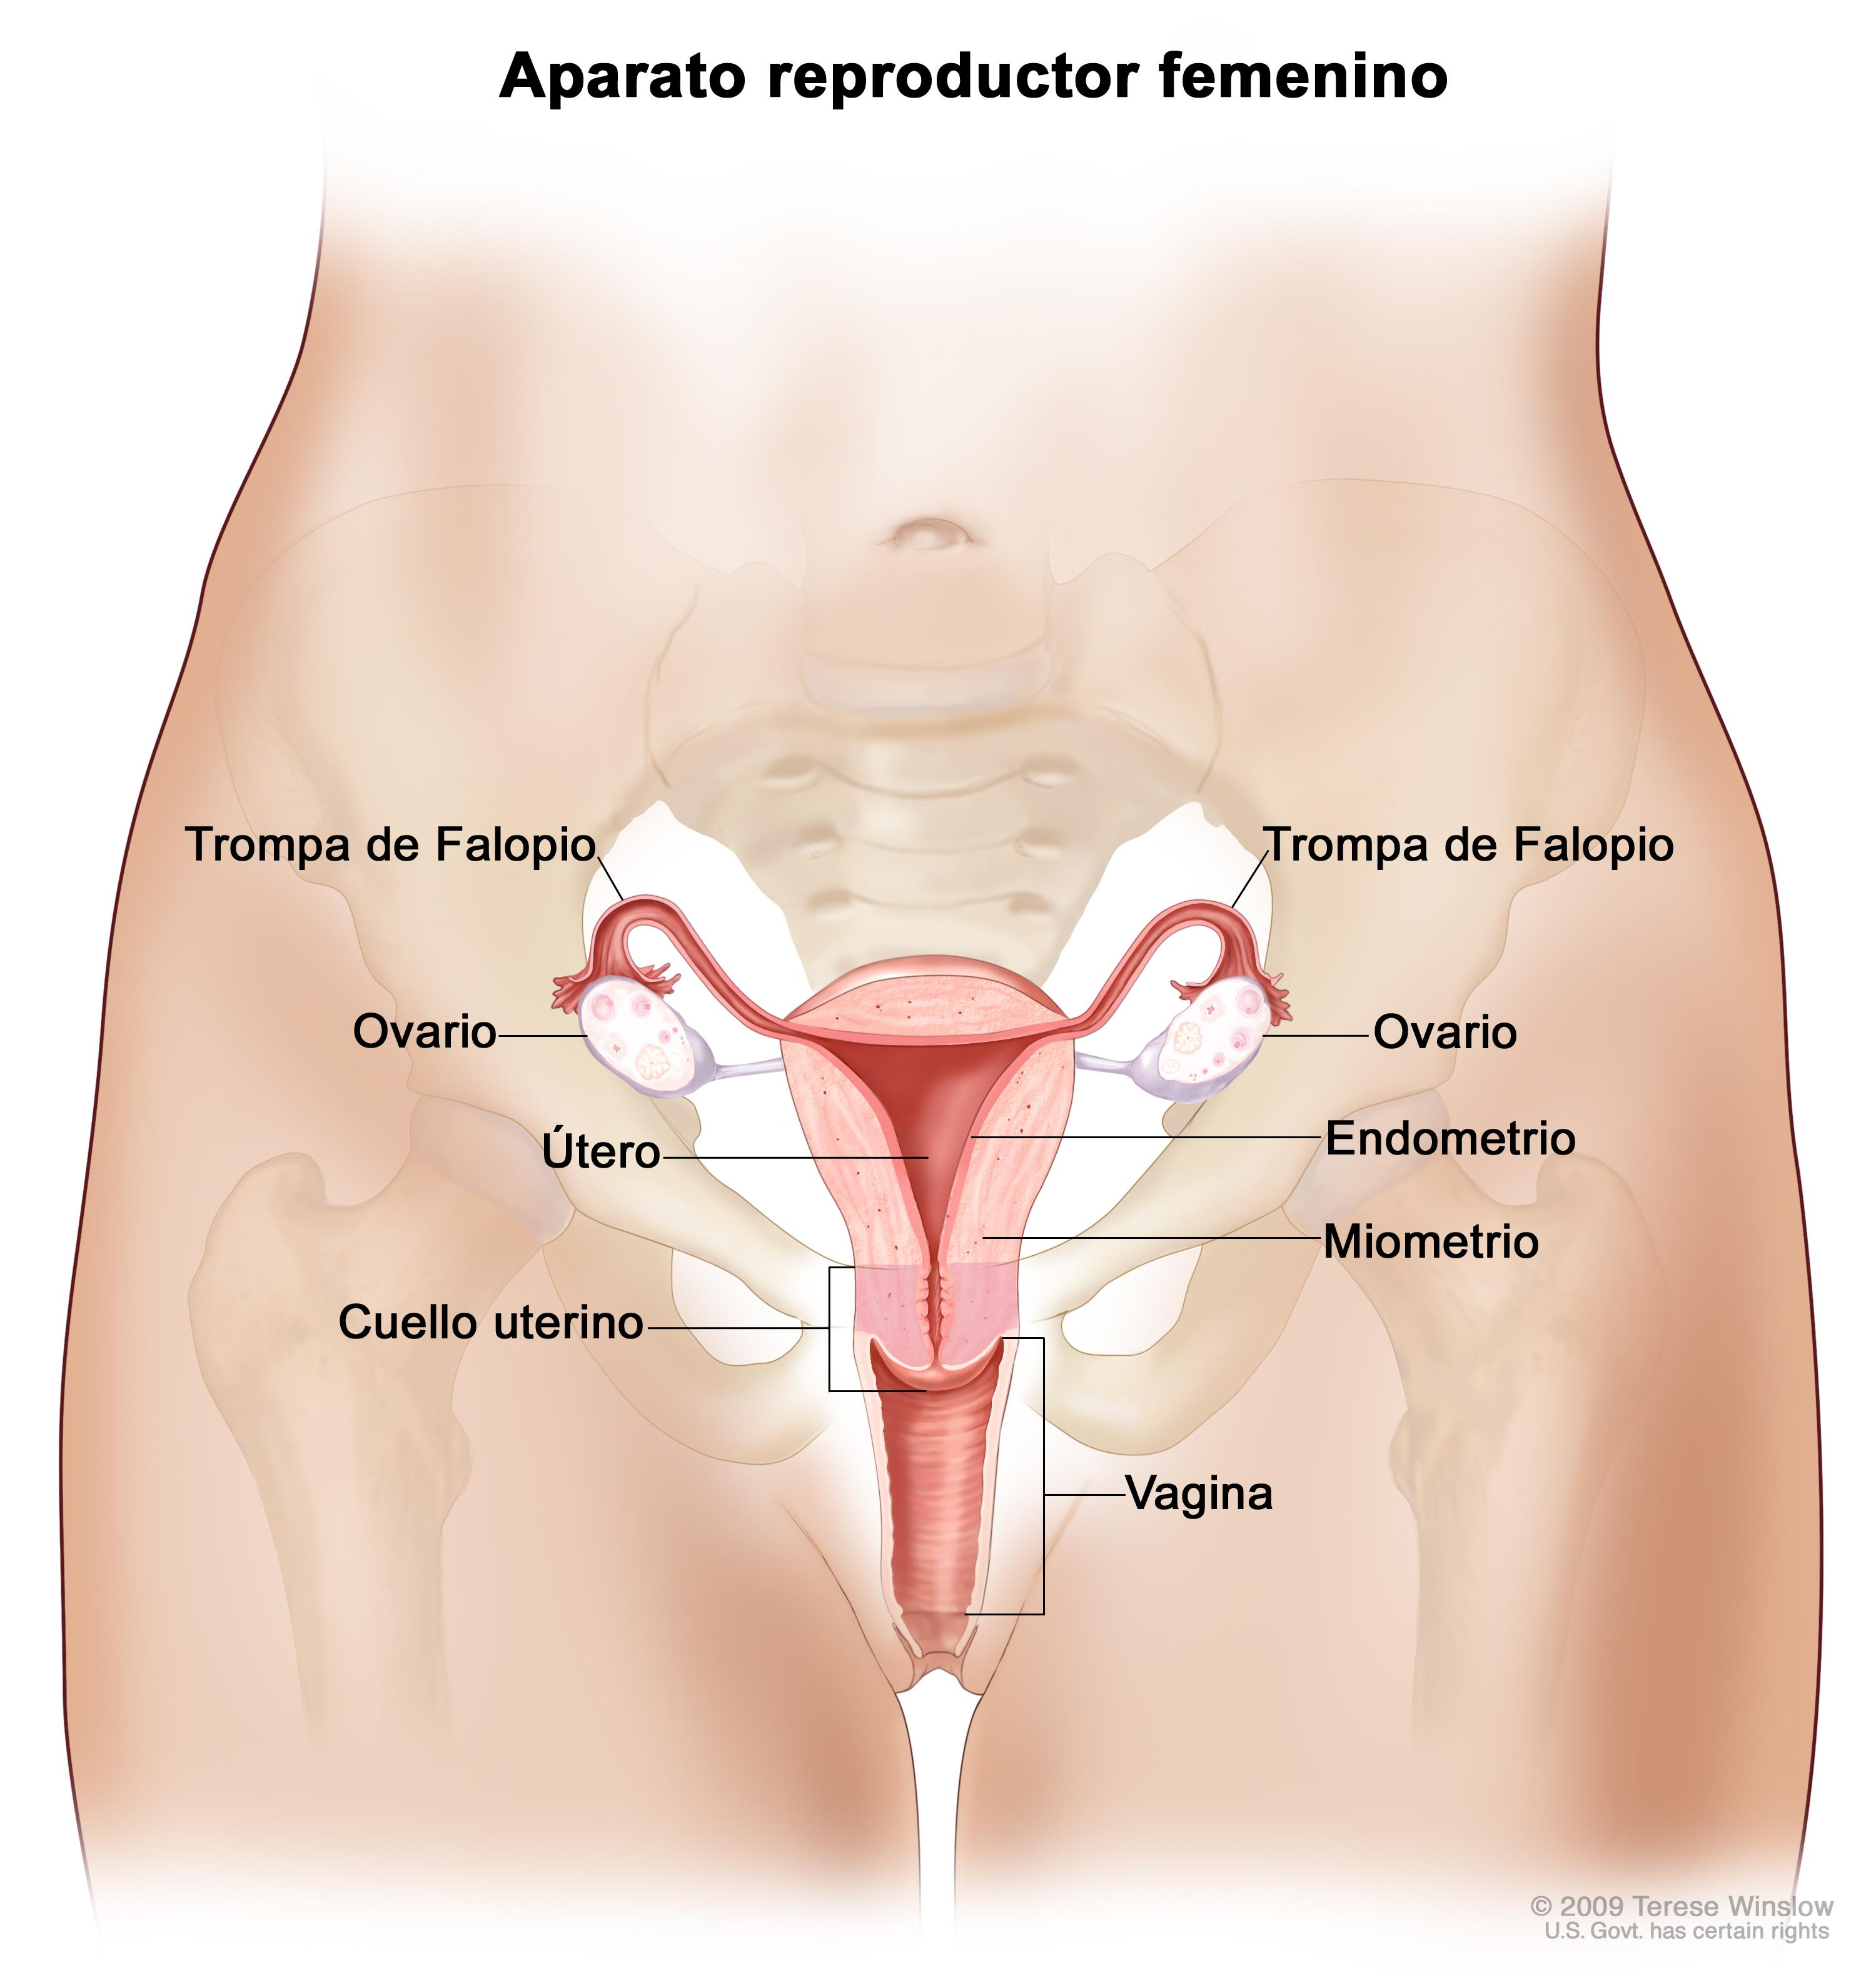
\includegraphics[scale=0.1]{capitulo_marcoteorico/cervix.jpg}
    \caption{Localización anatómica del cervix}\label{fig:cervix}
\end{figure}

%% \subsection{Características}

\subsubsection{Síntomas}

El cáncer cervical es sumamente peligroso debido a que sus primeros estados son
mayormente asintomáticos, es decir, no presentan síntomas visibles. En aquellas
pacientes con la suerte de presentar síntomas, el sangrado anormal durante el
coito, intermenstrual o irregularidades en el flujo de su menstruación son las
manifestaciones más comunes; esta pérdida de sangre inclusive puede desencadenar
cuadros de anemia. Es en sus estados avanzados donde se puede presentar
supuraciones anormales. Es cuando el tumor ha alcanzado un tamaño considerable
que empieza a ejercer presión en los órganos, tejidos y nervios  adyacentes, es
en esa etapa donde comienza el dolor. Otros síntomas morfológicos incluyen
sangrado por el recto y sangre en la orina, problemas circulatorios en ambas
piernas. 

Los síntomas que busca el médico en el historial de una paciente con evidencia de cáncer
son los siguientes. 

\begin{itemize}
    \item Sangrado intermenstrual.
    \item Sangrado postcoital.
    \item Modificación de patrones menstruales.
    \item Sangrado postmenopausia.
    \item Hiper-mucosidad.
    \item Dolor pélvico.
    \item Dolor coital.
\end{itemize}

\subsubsection{Desarrollo}

El cáncer de cérvix no aparece instantáneamente. Se manifiesta a través de
cambios graduales de las células que las van cambiando por una gama de etapas
tales como la Neoplasia Cervical Intraepitelial, Lesión Escamosa Intraepitelial,
Displasia, Hiperplasia etcétera.~\cite{NacionalCancerInstitute2012}

En la~\autoref{fig:desarrollo} se da una comparativa entre cuatro etapas del
cáncer. La etapa normal no muestra ninguna lesión visible, la lesión de grado
bajo comienza a mostrar cambios morfológicos; la diferencia entre las últimas
dos etapas es mínima pero importante, una lesión precancerosa conlleva al cáncer
pero no tiene los efectos tan devastadores en el cuerpo como un cáncer ya
formado..

\begin{figure}[H]
    \centering
    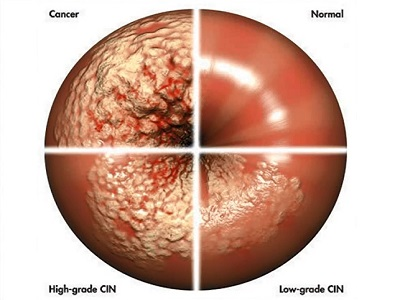
\includegraphics[width=0.6\textwidth]{capitulo_marcoteorico/cancer2.jpg}
    \caption{Desarrollo del cáncer}\label{fig:desarrollo}
\end{figure}


\subsection{Epidemiología}

Del \hyperlink{abbr}{CCU}, la Secretaria de Salud nos da los siguientes datos
sobre su epidemiología:“El cáncer del cuello uterino es la séptima neoplasia más
frecuente en la población mundial y la cuarta más frecuente entre las mujeres
con un estimado de 528mil nuevos casos diagnosticados anualmente, 85\% de los
cuales se registran en países en vías de desarrollo. La incidencia es más alta
en países en vías de desarrollo; varía desde 42.7 en África Oriental, hasta 4.4
por 100,000 mujeres en Asia occidental (Medio oriente). Es también una
importante causa de muerte por un tumor maligno en la mujer con 266,000
defunciones anuales, 87\% de las cuales ocurren en países subdesarrollados. Las
tasas de mortalidad que van de 2 en Asia Occidental a 27.6 defunciones por
100,000 mujeres en África Oriental. Mientras que en México, el
\hyperlink{abbr}{CCU} es la segunda causa de muerte por cáncer en la mujer. Más
de 13960 casos se detectan anualmente, esto genera una incidencia de 23.3 casos
por cada 100000 mujeres. La muerte por \hyperlink{abbr}{CCU} es un fuerte
indicador de un país en subdesarrollo o en desarrollo, es imperativo para las
políticas nacionales de sanidad la búsqueda de la erradicación de este
padecimiento. Actualmente, se sabe que la mayoría de los casos de
\hyperlink{abbr}{CCU} son detonados por una infección del Virus del Papiloma
Humano y que, a futuro, se pueda encontrar una solución al problema en forma de
alguna vacuna. Mientras tanto, todos los esfuerzos se deben enfocar en la
detección temprana y precisa.~\cite{SecretariadeSalud2015a}

En el mundo, este cáncer es el tercer tipo de cáncer más común y la cuarta causa
de muerte en las mujeres. En 2008, más de medio millón de casos fueron
diagnosticados. Con la introducción de la prueba de Papanicolau, se ha reducido
la incidencia y mortalidad, así como la tasa de canceres invasivos en alrededor
de 75\% en un periodo de alrededor de 50 años, lamentablemente, el 86\% de los
casos ocurren en países en vías de desarrollo, como México. Así mismo, la
incidencia del este tipo de cáncer es mayor en grupos de población vulnerables,
como gente en condición de pobreza y pobreza extrema, así como indígenas e
inmigrantes. En contraste con los países desarrollados, donde el riesgo de
padecer cáncer es de 0.9\%, mientras que la tasa de mortalidad es de 0.3\%; en
países como México, el riesgo de padecer es de 1.9\% y el de fallecer es de
1.1\%. Una cifra inaceptable para cualquier estándar mínimo de calidad de vida
humana.


\subsubsection{Factores de riesgo}
% poner que causa el virus verrugas y cosas así
Como todo cáncer, los factores externos inciden directamente en la probabilidad
de adquirirlo. En el caso del cáncer cervical, el Virus del Papiloma Humano
(\hyperlink{abbr}{VPH}\nomenclature{VPH}{Virus del Papiloma Humano})\index{Virus
del Papiloma Humano} es el factor de riesgo más prominente, donde más del 99\%
de los casos contienen restos de ADN de este virus.
% este virus. Una representación gráfica del virus puede encontrarse en la~\autoref{fig:virus}.

% \begin{figure}[H]
%     \centering
%     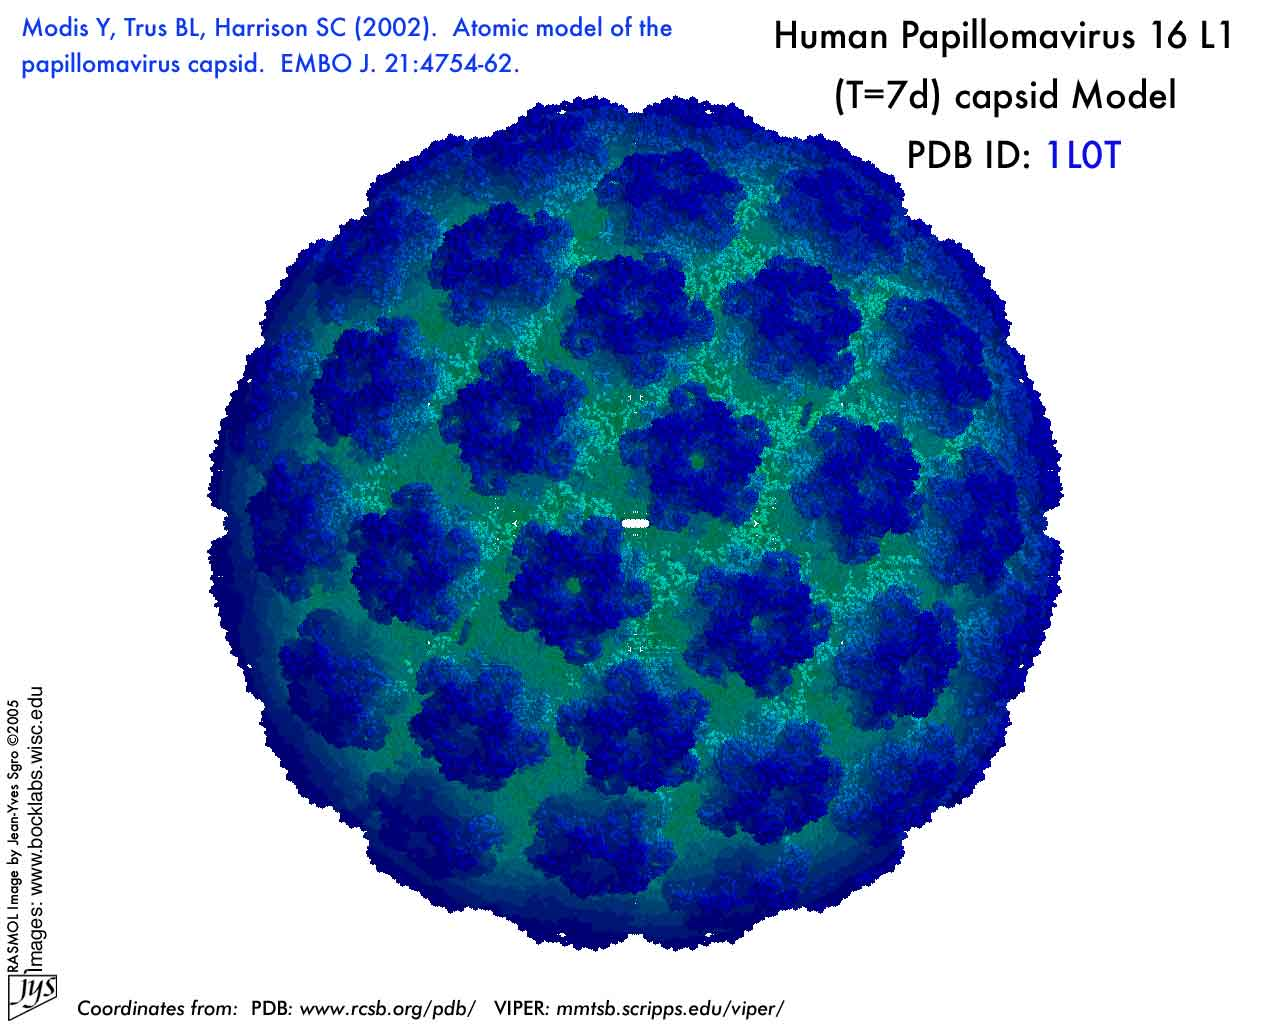
\includegraphics[scale=0.3]{capitulo_marcoteorico/virus.jpg}
%     \caption{Virus del Papiloma Humano}\label{fig:virus}
% \end{figure}

Existen más de 40 variedades del virus y la mayoría de ellas son capaces de
infectar a las mujeres en su tracto genital, lo preocupante de ello es que al
menos 15 de estas variedades se han demostrado como generadoras de  lesiones que
posteriormente se manifestarán como cáncer. La capacidad oncogénica de estos
virus cambia de tipo en tipo y algunos pueden resultar ser más agresivos que
otros. 

Aunque la epidemiología del \hyperlink{abbr}{VPH} difiere de la del cáncer, su
correlación con la del cáncer es obvia. La prevalencia del \hyperlink{abbr}{VPH}
en países con alta incidencia de casos de cáncer es de 10\% a 20\%, si la
comparamos con los países donde hay una incidencia baja de cáncer, esta es de
5\% a 10\%, se observa una variación significativa. 

El mecanismo por el cual el \hyperlink{abbr}{VPH} genera el cáncer está
relacionado con la interacción de ciertas proteínas con unos genes que inhiben
el crecimiento tumoral. Es esta pérdida del mecanismo regulador propio del
cuerpo que permite que las lesiones morfológicas deriven en cáncer. Es por ello
que el riesgo de cáncer invasivo está estrechamente relacionado con la
exposición de este virus y puede ser perturbado por el estado del sistema
inmunológico del paciente en particular\footnote{Es por ello que su incidencia
es mayor en personas inmunodeprimidas.}. 

Los riesgos demográficos a nivel mundial incluyen la raza, el estado
socioeconómico, el índice de desarrollo humano del país y lo robusto de su
sistema de salud. El estilo de vida de la persona también influye en el riesgo;
factores relacionados con el coito, cantidad de parejas sexuales, otras
enfermedades sexuales, mientras que el fumar multiplica la probabilidad por
cuatro y acelera la velocidad en que se desarrolla el cáncer. Más factores como
la cantidad de hijos, el uso de anticonceptivos, trasplante renal y el SIDA
también confabulan para incrementar el riesgo de padecer esta enfermedad.

\subsubsection{Mortalidad}
El pronóstico de una persona que padece cáncer está gobernado por la etapa del
cáncer, si existen ganglios involucrados, el volumen del tumor, la profundidad
de la invasión, los vasos sanguíneos comprometidos y en menor grado, variables
histológicas. Después del estado del cáncer, los ganglios son el factor más
importante en la mortalidad y pronóstico de esta enfermedad; esto es debido a
que los ganglios pueden extender el cáncer a otros órganos tan lejanos como el
cerebro.

La tasa de supervivencia a 5 años es la siguiente:

\begin{itemize}
    \item Metástasis distante: 16\%
    \item Regional: 56\%
    \item Localizado: 92\%
    \item Sin etapa: 60\%
\end{itemize}

\subsection{Diagnóstico}

Como pudimos ver en la sección anterior, la supervivencia del cáncer es
muchísimo mayor cuanto más rápido se diagnostique. Las pruebas para detectar
este cáncer en las mujeres debe comenzar a partir de los 21 años. En las mujeres
de 30 a 65 años, la prueba no solo debe de ser por cáncer, sino también para
\hyperlink{abbr}{VPH} y debe ser realizada cada 5 años. Las mujeres de entre 21
y 29 años, por su vida sexual, deben de realizar la prueba cada 3 años de
preferencia. Estas pruebas generalmente terminan a los 65 años si la mujer
cumple ciertos requisitos.

Los estudios citológicos realizados para buscar signos de cáncer deben estar
estandarizados bajo el esquema de Bethesda~\cite{Kurman1995}. La interpretación
está dividida en dos clases: hallazgos no malignos y anormalidades celulares
epiteliales donde se incluyen células escamosas y glandulares. En particular, la
prueba de Papanicolaou es inadecuada para la búsqueda de lesiones precursoras de
adenocarcinoma, es por ello que nos enfocaremos en las lesiones en células
escamosas. La~\autoref{fig:celu} nos da una comparativa entre ambos tipos
de células, escamosas y glandulares. 


\begin{figure}[H]
    \centering
    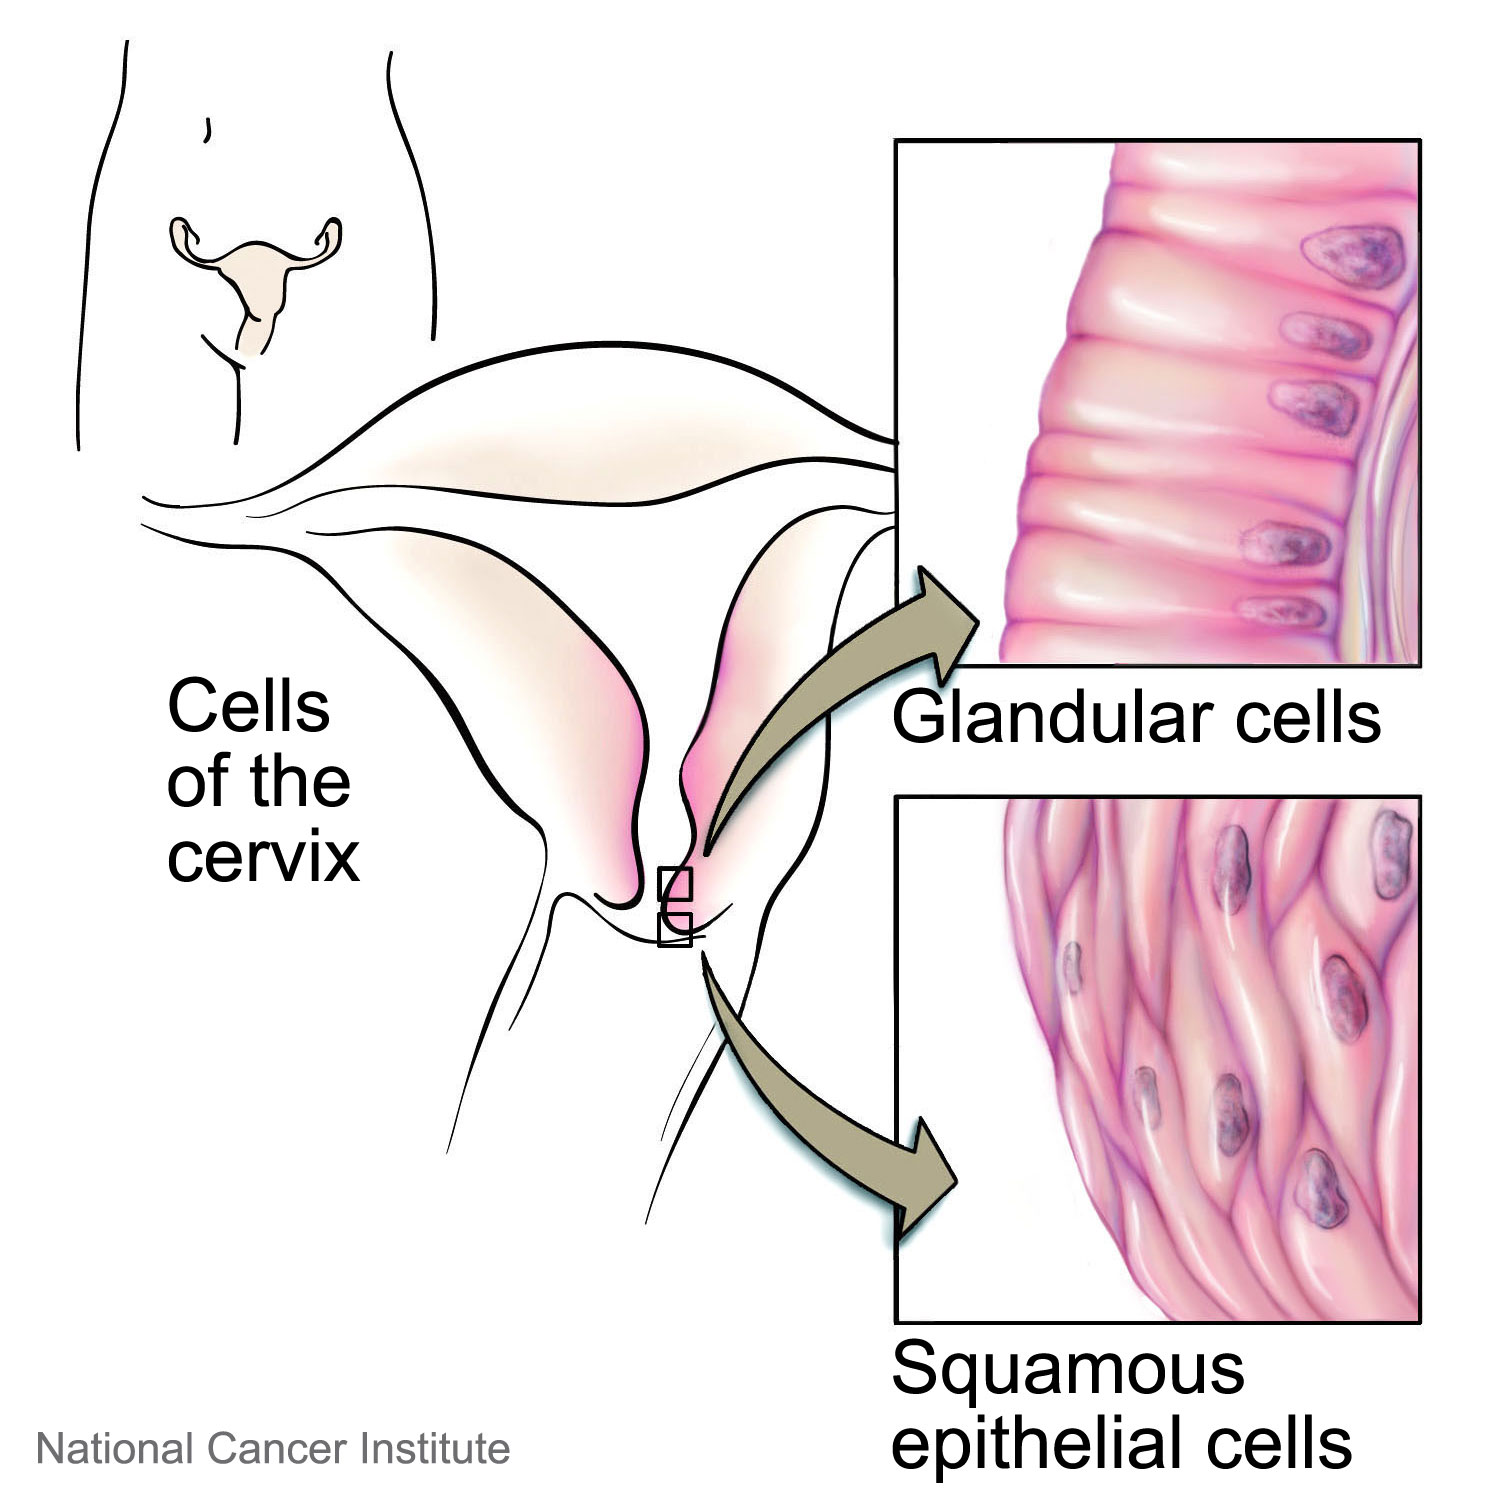
\includegraphics[scale=0.15]{capitulo_marcoteorico/celulas.jpg}
    \caption{Comparativa entre células del cérvix}\label{fig:celu}
\end{figure}

El \hyperlink{abbr}{CCU} se diagnostica aplicando una variedad de pruebas que
analizan la integridad de células y tejidos dentro del cérvix de la mujer.
Varias técnicas se muestran en la~\autoref{tabla:tecnicas}:

\begin{table}[H]
    \centering
    \resizebox{\textwidth}{!}{%
    \begin{tabular}{@{}lllll@{}}
    \toprule
    Nombre               & Tipo        & Descripción
    &  &  \\ \midrule Colposcopia          & Observación &
    \begin{tabular}[c]{@{}l@{}}Se introduce un colposcopio dentro de la vagina
    de la mujer\\   para observar la reacción del cérvix ante estímulos como el
    ácido acético.\end{tabular}                               &  &  \\
    Raspado endocervical & Biopsia     & \begin{tabular}[c]{@{}l@{}}Se corta un
    pequeño\\   trozo del cérvix para su análisis bajo microscopio, se pretende
    analizar la\\   estructura del tejido.\end{tabular}
    &  &  \\
    Papanicolau          & Citología   & \begin{tabular}[c]{@{}l@{}}Se toma una
    muestra de las células cervicales y se\\   extienden en una laminilla que es
    examinada por el experto. Funge como criba\\   para pruebas más
    especializadas.\end{tabular} &  &  \\ \bottomrule \end{tabular}%
    }
    \caption{Técnicas principales de diagnóstico de CCU}\label{tabla:tecnicas}
    \end{table}

\subsubsection{Examen de Papanicolaou}

El examen de Papanicolau\index{Examen de Papanicolau}, creado en 1927, es la
prueba más usada en México debido a su facilidad de implementación y bajo costo,
con la desventaja que requiere más pericia del cito-tecnólogo para su
interpretación y que el acto de la toma de muestra puede inducir ruido y
dificultar el diagnóstico. 

Fue George Papanicolau uno de los pioneros en la ciencia de diagnosticar cáncer
con base en análisis de laminillas con células. Nacido en 1883 en Grecia, realizó
estudios universitarios en música y humanidades, siendo su padre el que eventualmente
lo persuadió en buscar una carrera médica, la cual concluyó con altos honores.

En 1920 se enfocó en la cito-patología del sistema reproductivo humano donde se
maravilló al encontrar diferencias morfológicas visibles entre las células
normales y las malignas. Fue en 1943 cuando publicó su libro más influyente que
catapultó su método a convertirse en el estándar de diagnóstico.~\cite{Tan2015}

Es un procedimiento en el cual un pequeño cepillo o espátula es usado para
remover células del cervix para poder ser analizadas bajo un microscopio en
busca de anormalidades como el cáncer o las lesiones precursoras del mismo. Una
prueba de Papanicolau también permite encontrar infecciones o inflamación. En
la~\autoref{fig:papsmear} podemos observar un esquema simplificado con los tres pasos
del procedimiento.~\cite{NationalCancerInstitutea}
% citar
% https://www.medicalcenter.virginia.edu/medlabs/lab-tests/cytology/gyenocologic-pap-test-collection-procedure.html
\begin{figure}[H]
    \centering
    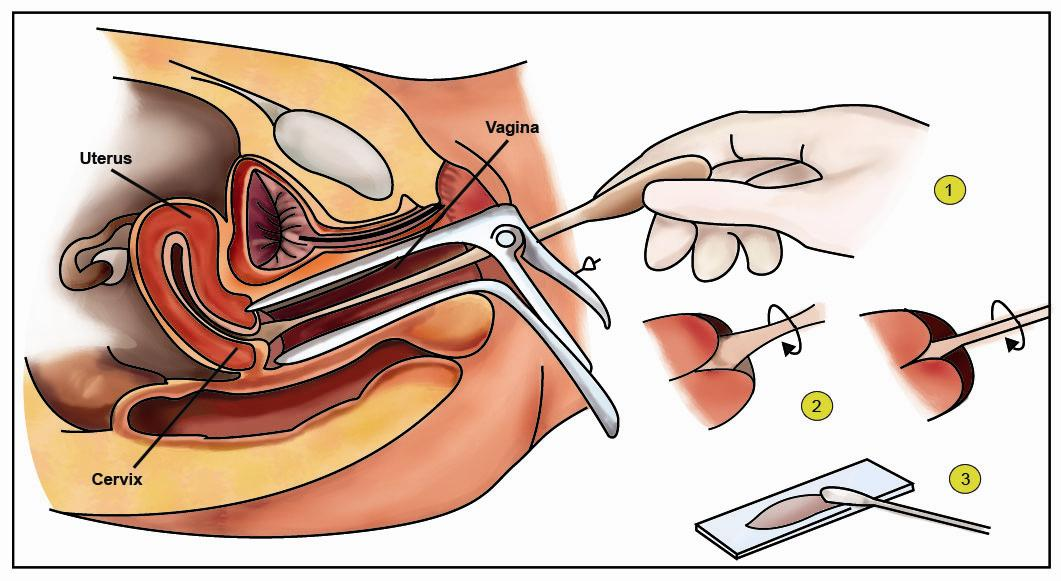
\includegraphics[width=0.7\textwidth]{capitulo_marcoteorico/papsmear.jpg}
    \caption{Prueba de Papanicolau}\label{fig:papsmear}
\end{figure}

Al concluir la toma de la muestra, esta se coloca en un portaobjetos para luego
ser analizada por el experto cito-tecnólogo. Existen varias formas de realizar
la preparación de la muestra; esta preparación si bien está sujeta a las
especificaciones tanto de la prueba como del sistema de diagnóstico, puede
variar debido a la pericia del personal que la realiza. En la~\autoref{fig:pap}
el resultado de la prueba de Papanicolaou, donde se observan bien diferenciadas
las células junto con sus organelos y componentes.

\begin{figure}[H]
    \centering
    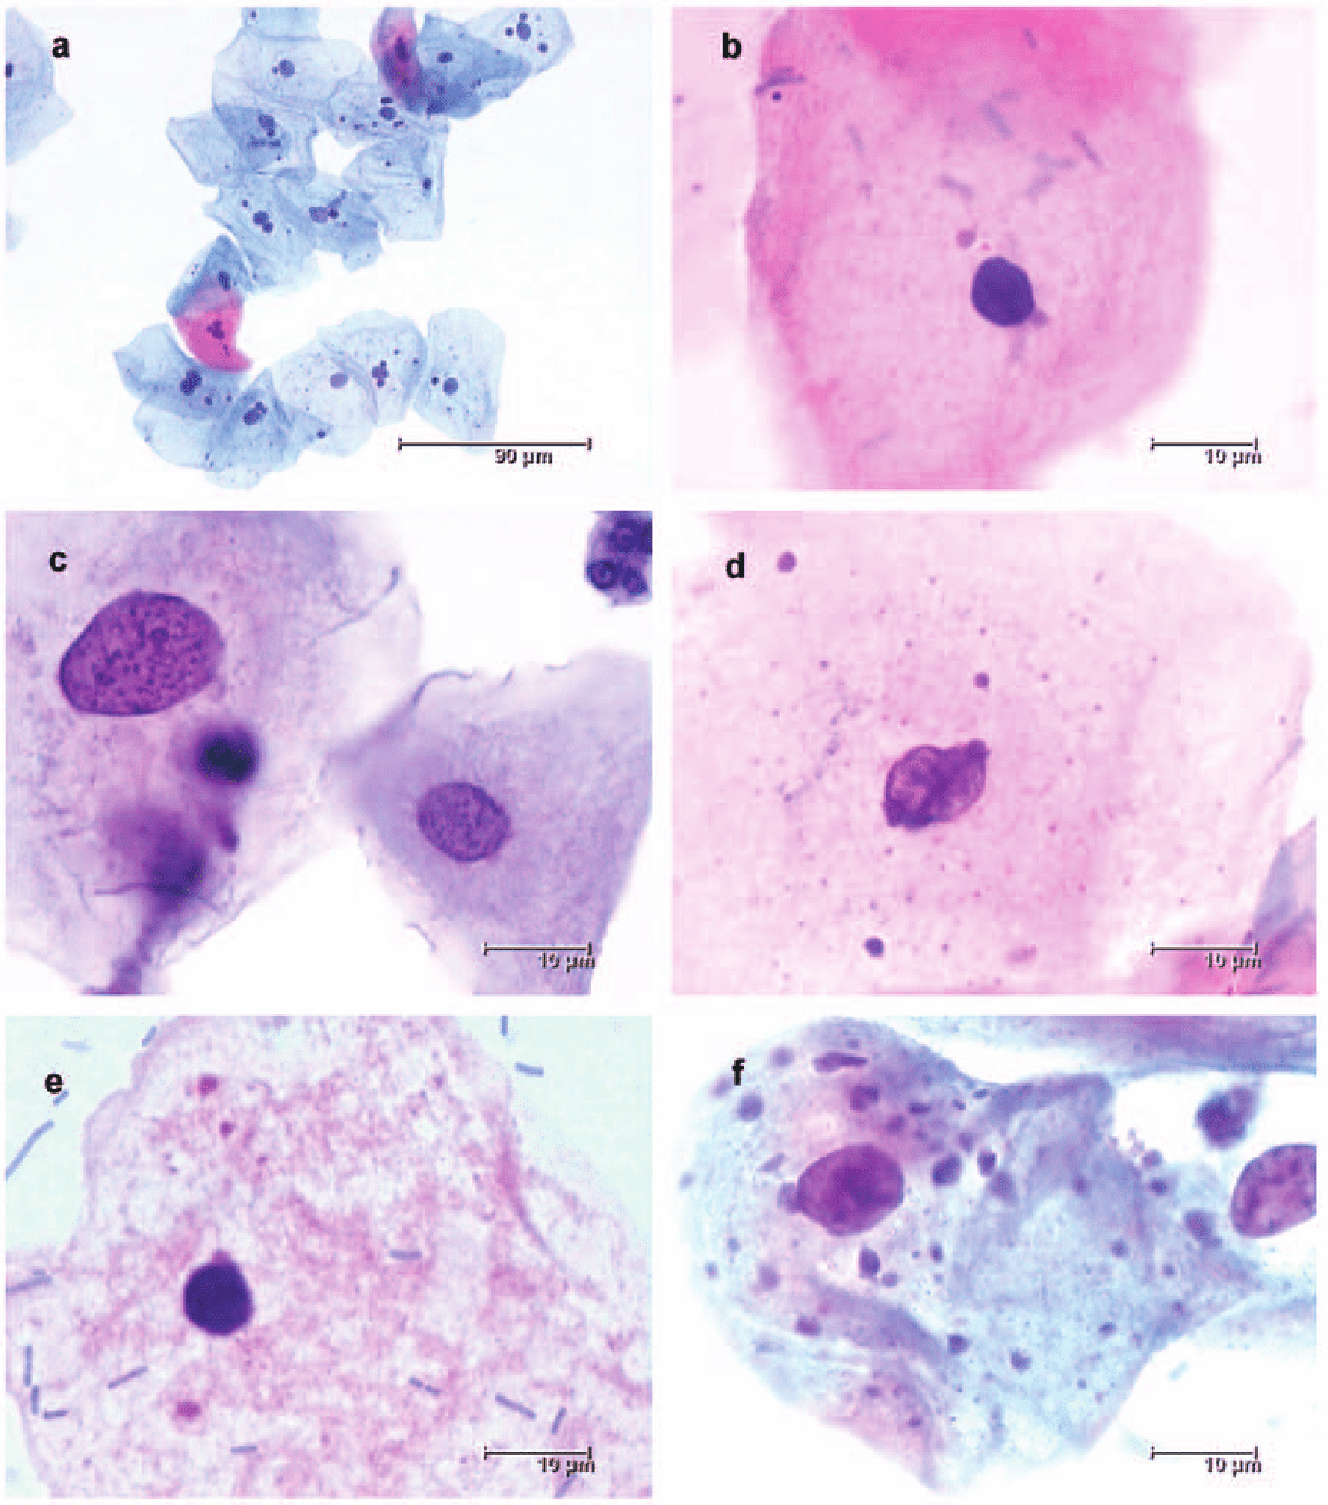
\includegraphics[scale=0.3]{capitulo_marcoteorico/pap.pdf}
    \caption{Prueba de Papanicolau: resultados}\label{fig:pap}
\end{figure}

\subsubsection{\emph{Bethesda System}}

Debido a la variabilidad en la implementación de la prueba de Papanicolau, que
incluye tanto la paciente, la pericia del tomador de la muestra, la mezcla
exacta de los reactivos y diluyentes, se creó un sistema que estandariza el
cribado de cáncer de cérvix. Este sistema se llama Bethesda\index{Sistema
\emph{Bethesda}}, por la ciudad de Maryland donde se llevó a cabo la conferencia
que acordó la creación de este sistema. Este sistema clasifica los resultados de
la observación de la muestra de Papanicolau de la siguiente manera, que se
muestra en la~\autoref{tabla:bethesda}:

\begin{table}[H]
    \centering
    \resizebox{0.6\textwidth}{!}{%
    \begin{tabular}{@{}ll@{}}
    \toprule
    Nomenclatura & Significado                                         \\
    \midrule ASC US       & Células escamosas atípicas de significado incierto
    \\
    ASC H        & Células escamosas atípicas sugestivas de alto grado \\
    AGC          & Células Glandulares Atípicas                        \\
    LSIL         & Lesión intraepitelial escamosa de bajo grado        \\
    HSIL         & Lesión intraepitelial escamosa de alto grado         \\
    ACIS         & Adenocarcinoma in situ (endocervical)               \\
    \bottomrule \end{tabular}%
    }
    \caption{Niveles del sistema Bethesda de reporte cervical y citológico}\label{tabla:bethesda}
    \end{table}

Para la identificación y clasificación de estas etapas, se buscan
características celulares que sean indicadoras de cambios morfológicos
(\autoref{fig:ciclo}). Estos indicadores tienen que ver con las características
físicas de la célula y los organelos que la componen. Características tales como
el tamaño del núcleo, el citoplasma, la relación entre estos, el tamaño de la
célula, características de la membrana etcétera, fungen como elementos decisores
para clasificar cada célula en particular para ajustarla al sistema Bethesda.
Condiciones ambientales del área y herramientas de trabajo del cito-tecnólogo,
como las características del microscopio, la concentración de los diluyentes,
temperatura, estado mental, estado físico (visión cansada), cantidad de trabajo;
inciden negativamente en la tasa de diagnóstico. El problema más grave se
presenta cuando el departamento de citología presenta una afluencia grande de
muestras que requieren procesamiento, sin embargo, por las características del
trabajo, se tiene una limitación de cuantas muestras pueden ser analizadas por
día.~\cite{Kurman1995}

\begin{figure}[H]
    \centering
    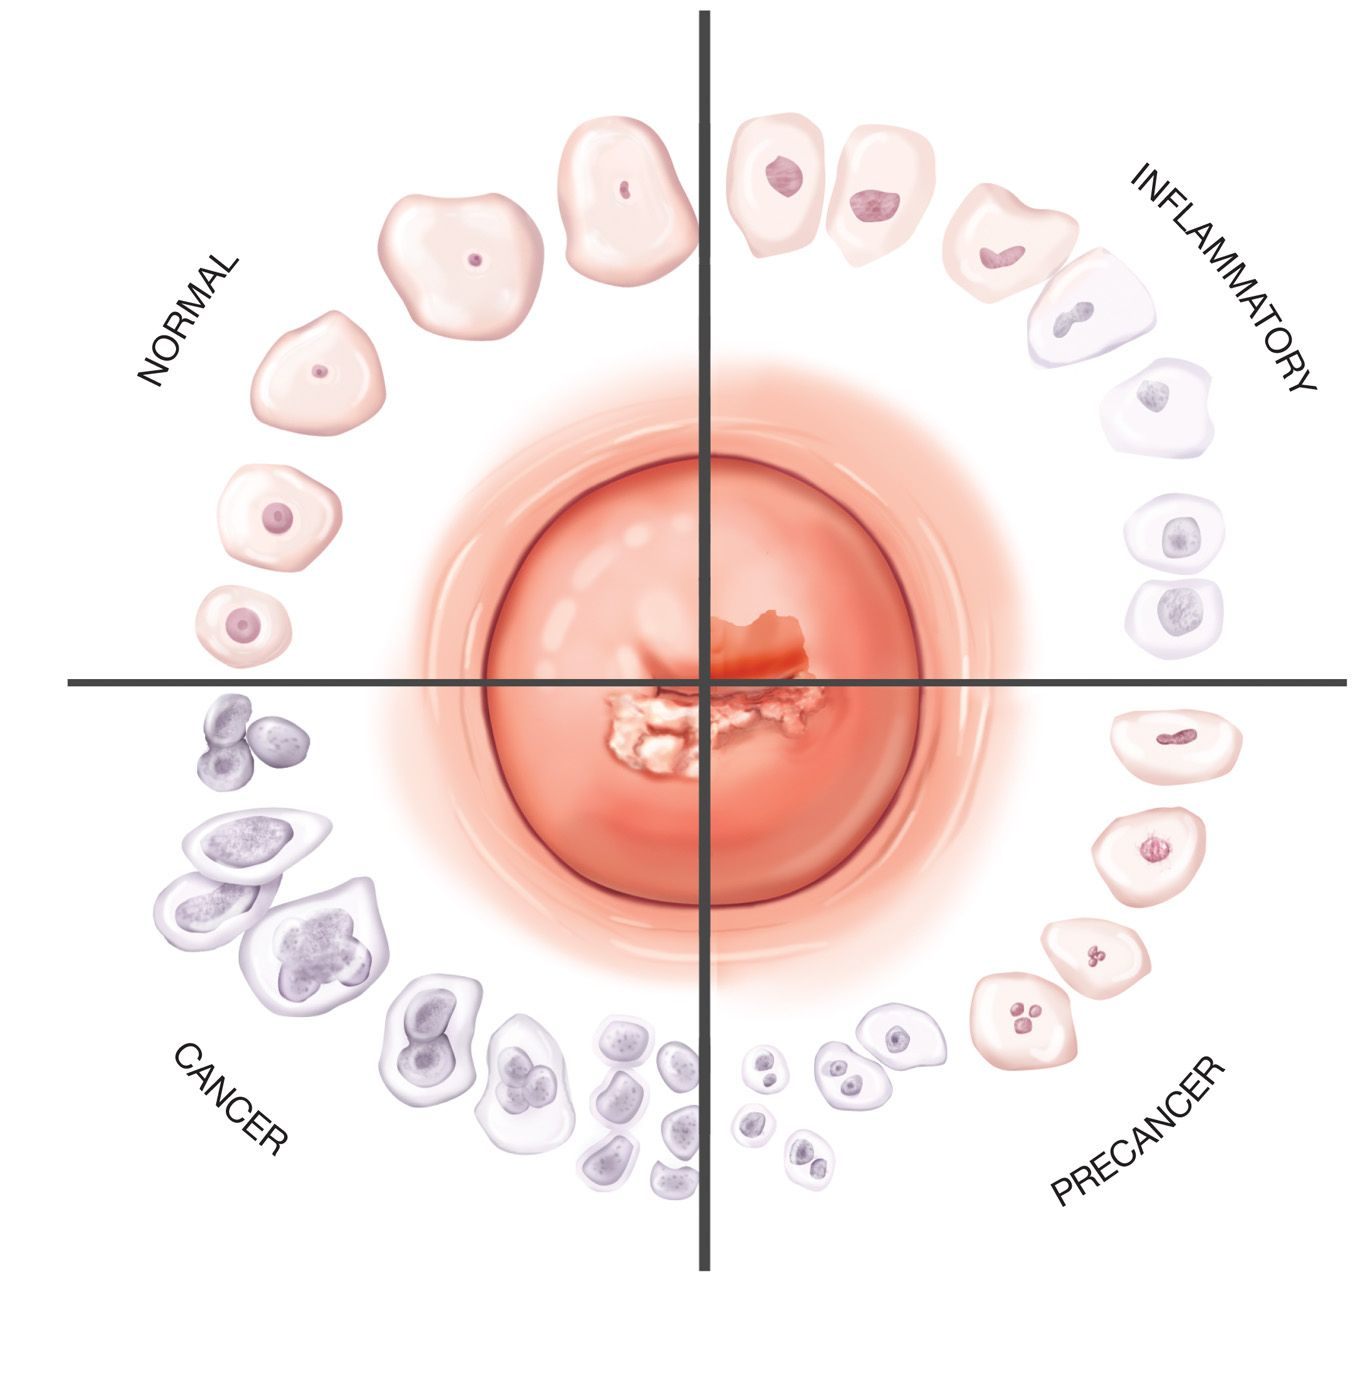
\includegraphics[scale=0.15]{capitulo_marcoteorico/ciclo.jpg}
    \caption{Ciclo de displasia celular y su relación con el cérvix}\label{fig:ciclo}
\end{figure}